%-----BEGIN DISCLAIMER-----
%******************************************************************************
% Copyright (c) 2011, 2020 JCrypTool Team and Contributors
%
% All rights reserved. This program and the accompanying materials
% are made available under the terms of the Eclipse Public License v1.0
% which accompanies this distribution, and is available at
% http://www.eclipse.org/legal/epl-v10.html
%******************************************************************************
%-----END DISCLAIMER-----

% This is a redraw of an old pixel graphic in svg vector format for the
% online help of the JCrypTool plug-in "Multipartite Key Exchange".
%
% To build the svg, you require: 
%
%  * a LaTeX distribution (https://latex-project.org/)
%  * the TikZ/PGF package (https://ctan.org/pkg/pgf)
%  * ImageMagick's convert on path (https://imagemagick.org/)
%
% If requirements are fulfilled, run following command:
% pdflatex --shell-escape multipartite-graph.tex

\documentclass[tikz, convert=pdf2svg]{standalone}
\begin{document}
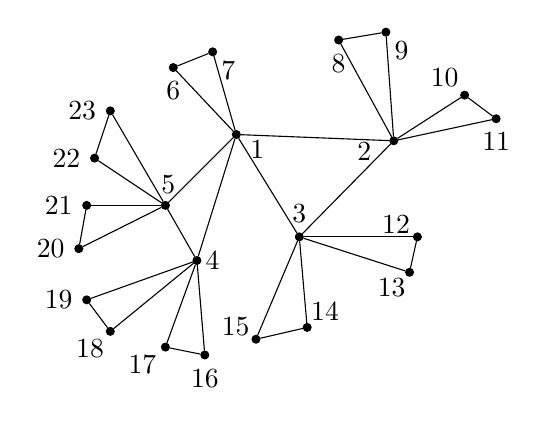
\begin{tikzpicture}

    % Define the circle size of the graph's nodes.
    \pgfmathsetmacro{\sepValue}{1}

    %% ------
    %% Start do draw nodes and arrows
    %% The nodes are positioned on fixed coordinates
    %% (sorry for that one)
    %% Some minor details are adjusted manually
    %% with [label distance] and [xshift/yshift]
    %% ----

    % 1
    \node[draw, circle, fill=black, color=black, inner sep=\sepValue, label={[yshift=2pt] -20:1}] (1) {};

    % 6 - 7
    \node[draw, circle, fill=black, color=black, inner sep=\sepValue, label={269:6}] (6) at (-0.8, 0.85) {};
    \node[draw, circle, fill=black, color=black, inner sep=\sepValue, label={[label distance=-2pt] -20:7}] (7) at (-0.3, 1.05) {};
    \draw[-] (6) -- (7);
    \draw[-] (1) -- (6);
    \draw[-] (1) -- (7);

    %2 
    \node[draw, circle, fill=black, color=black, inner sep=\sepValue, label={[yshift=-4pt, xshift=-3pt] 182:2}] (2) at (2, -0.08) {};
    \draw[-] (1) -- (2);

    % 8 - 9
    \node[draw, circle, fill=black, color=black, inner sep=\sepValue, label={269:8}] (8) at (1.3, 1.2) {};
    \node[draw, circle, fill=black, color=black, inner sep=\sepValue, label={[label distance=-2pt] -20:9}] (9) at (1.9, 1.3) {};
    \draw[-] (8) -- (9);
    \draw[-] (2) -- (8);
    \draw[-] (2) -- (9);

    % 10 - 11
    \node[draw, circle, fill=black, color=black, inner sep=\sepValue, label={[label distance=-3pt] 160:10}] (10) at (2.9, 0.5) {};
    \node[draw,, circle, fill=black, color=black, inner sep=\sepValue, label={270:11}] (11) at (3.3, 0.2) {};
    \draw[-] (10) -- (11);
    \draw[-] (2) -- (10);
    \draw[-] (2) -- (11);
    
    % 5 
    \node[draw,, circle, fill=black, color=black, inner sep=\sepValue, label={[label distance=-1pt, xshift=1pt] 90:5}] (5) at (-0.9, -0.9) {};
    \draw[-] (1) -- (5);

    % 22 - 23
    \node[draw, circle, fill=black, color=black, inner sep=\sepValue, label={181:22}] (22) at (-1.8, -0.3) {};
    \node[draw, circle, fill=black, color=black, inner sep=\sepValue, label={180:23}] (23) at (-1.6, 0.3) {};
    \draw[-] (22) -- (23);
    \draw[-] (5) -- (22);
    \draw[-] (5) -- (23);
    
    % 20 - 21  
    \node[draw, circle, fill=black, color=black, inner sep=\sepValue, label={180:20}] (20) at (-2, -1.45) {};
    \node[draw, circle, fill=black, color=black, inner sep=\sepValue, label={180:21}] (21) at (-1.9, -0.9) {};
    \draw[-] (20) -- (21);
    \draw[-] (5) -- (20);
    \draw[-] (5) -- (21);

    % 4 
    \node[draw, circle, fill=black, color=black, inner sep=\sepValue, label={[label distance=-2pt] 0:4}] (4) at (-0.5, -1.6) {};
    \draw[-] (1) -- (4);
    \draw[-] (4) -- (5);

    % 18 - 19
    \node[draw, circle, fill=black, color=black, inner sep=\sepValue, label={[label distance=-3pt] 210:18}] (18) at (-1.6, -2.5) {};
    \node[draw, circle, fill=black, color=black, inner sep=\sepValue, label={180:19}] (19) at (-1.9, -2.1) {};
    \draw[-] (18) -- (19);
    \draw[-] (4) -- (18);
    \draw[-] (4) -- (19);

    % 16 - 17
    \node[draw, circle, fill=black, color=black, inner sep=\sepValue, label={271:16}] (16) at (-0.4, -2.8) {};
    \node[draw, circle, fill=black, color=black, inner sep=\sepValue, label={[label distance=-2pt] 240:17}] (17) at (-0.9, -2.7) {};
    \draw[-] (16) -- (17);
    \draw[-] (4) -- (16);
    \draw[-] (4) -- (17);

    % 3 
    \node[draw, circle, fill=black, color=black, inner sep=\sepValue, label={90:3}] (3) at (0.8, -1.3) {};
    \draw[-] (1) -- (3);
    \draw[-] (2) -- (3);
    
    % 14 - 15
    \node[draw, circle, fill=black, color=black, inner sep=\sepValue, label={[label distance=-4pt] 30:14}] (14) at (0.9, -2.45) {};
    \node[draw, circle, fill=black, color=black, inner sep=\sepValue, label={[label distance=-4pt]120:15}] (15) at (0.25, -2.6) {};
    \draw[-] (14) -- (15);
    \draw[-] (3) -- (14);
    \draw[-] (3) -- (15);

    % 12 - 13
    \node[draw,, circle, fill=black, color=black, inner sep=\sepValue, label={[label distance=-4pt] 110:12}] (12) at (2.3, -1.3) {};
    \node[draw,, circle, fill=black, color=black, inner sep=\sepValue, label={[label distance=-4pt] 210:13}] (13) at (2.2, -1.75) {};
    \draw[-] (12) -- (13);
    \draw[-] (3) -- (12);
    \draw[-] (3) -- (13);

\end{tikzpicture}
\end{document}
